\documentclass[12pt,a4paper]{report}

% =========================================================================
% THU VIEN VA DINH DANG
% =========================================================================
\usepackage{fontspec}
\setmainfont{Times New Roman}
\usepackage[top=2.5cm,bottom=2.5cm,left=3.0cm,right=2.0cm]{geometry}
\usepackage{amsmath,amsfonts,amssymb}
\usepackage{graphicx}
\usepackage{booktabs,tabularx,multirow,array}
\usepackage{float}
\usepackage{xcolor}
\usepackage{tikz}
\usetikzlibrary{calc,positioning,shapes.geometric,arrows.meta}
\usepackage{pgfornament}
\usepackage{setspace}
\usepackage{hyperref}
\usepackage{fancyhdr}
\usepackage{titlesec}
\usepackage{caption}
\usepackage{subcaption}
\usepackage{enumitem}
\usepackage{listings}
\usepackage{tcolorbox}

\graphicspath{{images/generated/}{images/}}
\renewcommand{\arraystretch}{1.12}
\renewcommand{\contentsname}{Mục lục}
\renewcommand{\listfigurename}{Danh mục hình ảnh}
\renewcommand{\listtablename}{Danh mục bảng biểu}
\renewcommand{\chaptername}{Chương}
\renewcommand{\figurename}{Hình}
\renewcommand{\tablename}{Bảng}
\renewcommand{\lstlistingname}{Đoạn mã}

\hypersetup{
    colorlinks=true,
    linkcolor=black,
    citecolor=black,
    urlcolor=black,
    pdftitle={Bao Cao Ky Thuat Assignment 06 - RNN Forecasting va Localhost Deployment},
    pdfauthor={Duong Trong Thang}
}

\lstdefinestyle{mystyle}{
    backgroundcolor=\color{white},
    commentstyle=\color{black},
    keywordstyle=\color{black}\bfseries,
    numberstyle=\tiny\color{black},
    stringstyle=\color{black},
    basicstyle=\ttfamily\footnotesize\color{black},
    breakatwhitespace=false,
    breaklines=true,
    captionpos=b,
    keepspaces=true,
    numbers=left,
    numbersep=5pt,
    showspaces=false,
    showstringspaces=false,
    showtabs=false,
    tabsize=2,
    frame=single,
    rulecolor=\color{black}
}
\lstset{style=mystyle}

\titleformat{\chapter}[display]
  {\normalfont\bfseries\color{black}}
  {\filleft\Large\bfseries\chaptertitlename\ \thechapter}
  {1ex}
  {\titlerule\vspace{1ex}\filright\LARGE}
  [\vspace{1ex}\titlerule]
\titleformat{\section}
  {\normalfont\Large\bfseries\color{black}}
  {\thesection}{1em}{}
\titleformat{\subsection}
  {\normalfont\large\bfseries\color{black}}
  {\thesubsection}{1em}{}

\pagestyle{fancy}
\fancyhf{}
\fancyhead[R]{\small\itshape Assignment 06: RNN Forecasting và Localhost Deployment}
\fancyfoot[C]{\thepage}
\renewcommand{\headrulewidth}{0.4pt}
\renewcommand{\footrulewidth}{0.4pt}
\setlength{\headheight}{14pt}

\newcommand{\modelpath}[1]{\texttt{#1}}
\newcommand{\best}[1]{\textbf{#1}}
\newcommand{\codeinline}[1]{\texttt{#1}}
\newcommand{\safeimage}[3][\textwidth]{%
  \IfFileExists{images/generated/#2}{\includegraphics[width=#1]{#2}}{%
    \fbox{\parbox[c][6cm][c]{0.92\textwidth}{\centering\bfseries #3}}%
  }%
}

% Khung va logo trang bia, giu cung mau voi Assignment 05.
\newcommand{\decoratedframe}{%
  \begin{tikzpicture}[remember picture,overlay]
    \draw[line width=1.6pt]
      ($(current page.north west)+(1.2cm,-1.2cm)$) rectangle
      ($(current page.south east)+(-1.2cm,1.2cm)$);
    \draw[line width=0.8pt]
      ($(current page.north west)+(1.05cm,-1.05cm)$) rectangle
      ($(current page.south east)+(-1.05cm,1.05cm)$);
    \node[anchor=north west] at ($(current page.north west)+(1.18cm,-1.00cm)$)
      {\pgfornament[width=2.2cm]{61}};
    \node[anchor=north east] at ($(current page.north east)+(-1.18cm,-1.00cm)$)
      {\pgfornament[width=2.2cm,symmetry=v]{61}};
    \node[anchor=south west] at ($(current page.south west)+(1.18cm,1.00cm)$)
      {\pgfornament[width=2.2cm,symmetry=h]{61}};
    \node[anchor=south east] at ($(current page.south east)+(-1.18cm,1.00cm)$)
      {\pgfornament[width=2.2cm,symmetry=c]{61}};
  \end{tikzpicture}%
}

\newcommand{\fallbacklogo}{%
  
\begin{tikzpicture}
    \node[text=black,font=\bfseries\fontsize{34}{38}\selectfont,inner sep=1pt] (ptit) {PTIT};
    \node[star,star points=5,star point ratio=2.2,fill=black,draw=black,
      minimum size=0.78cm,inner sep=0pt] at ($(ptit.north)+(0.20cm,-0.06cm)$) {};
    \draw[black,line width=1.1pt]
      ($(ptit.south west)+(-0.10cm,-0.18cm)$) -- ($(ptit.south east)+(0.10cm,-0.18cm)$);
    \draw[black,line width=0.45pt]
      ($(ptit.south west)+(-0.10cm,-0.25cm)$) -- ($(ptit.south east)+(0.10cm,-0.25cm)$);
  \end{tikzpicture}%
}

\newcommand{\showlogo}{%
  \IfFileExists{images/generated/ptit.jpg}
    {
\includegraphics[width=4cm]{ptit.jpg}}
    {\fallbacklogo}%
}

\begin{document}
\color{black}

% =========================================================================
% TRANG BIA
% =========================================================================
\newgeometry{margin=2.2cm}
\hypersetup{pageanchor=false}
\begin{titlepage}
\setstretch{1.3}
\setlength{\parskip}{6pt}
\thispagestyle{empty}
\decoratedframe
\centering
\vspace*{1.2cm}

{\large\textbf{HỌC VIỆN CÔNG NGHỆ BƯU CHÍNH VIỄN THÔNG}}\\[4pt]
{\large\textbf{KHOA CÔNG NGHỆ THÔNG TIN 1}}\\[10pt]
\rule{7cm}{0.4pt}\\[0.8cm]

\showlogo\\[0.5cm]

{\huge\bfseries BÁO CÁO ASSIGNMENT 06}\\[10pt]
{\Large\bfseries MÔN HỌC: PHÁT TRIỂN HỆ THỐNG THÔNG MINH}\\[15pt]

{\textbf{Lớp D23CTPM01}}\\[6pt]
{\large\textbf{Giảng viên: Trần Đình Quế}}\\[0.8cm]

\begin{spacing}{1.2}
\setlength{\tabcolsep}{10pt}
\begin{tabular}{@{}>{\raggedright\arraybackslash}p{6.2cm} >{\raggedright\arraybackslash}p{4.2cm}@{}}
\textbf{Họ và Tên} & \textbf{Dương Trọng Thắng} \\
\textbf{Mã sinh viên} & \textbf{B23DCCN752} \\
\end{tabular}
\end{spacing}

\vfill
{\large\itshape Hà Nội -- 2026}
\end{titlepage}
\restoregeometry
\hypersetup{pageanchor=true}

\pagenumbering{roman}
\tableofcontents
\newpage
\listoffigures
\newpage
\listoftables
\newpage
\pagenumbering{arabic}

% =========================================================================
% THONG TIN PROJECT
% =========================================================================
\chapter*{Thông tin dự án}
\addcontentsline{toc}{chapter}{Thông tin dự án}
\noindent\textbf{GitHub project:} \url{https://github.com/duongthang2710/PTHTTM}

\vspace{0.4cm}
\noindent Assignment 06 được triển khai trên hai bài toán dự báo giá độc lập. Mã nguồn thực nghiệm nằm tại:
\begin{itemize}
    \item Amazon Stock Price:\\
    \modelpath{Assignment6/Amazon Stock Price/notebook/}\\
    \modelpath{amazon\_rnn\_forecasting.ipynb};
    \item Avocado Price:\\
    \modelpath{Assignment6/Avocado Price/notebook/}\\
    \modelpath{avocado\_rnn\_forecasting.ipynb}.
\end{itemize}

Mỗi notebook thực hiện trọn quy trình từ khảo sát dữ liệu, tạo cửa sổ thời gian, huấn luyện vanilla RNN
bằng PyTorch và Keras đến đánh giá trên tập test theo thứ tự thời gian. Các trọng số tốt nhất cùng tham số
chuẩn hóa được lưu để hai ứng dụng Flask có thể suy luận trực tiếp trên localhost. Hình minh họa và số liệu
trong báo cáo được lấy từ kết quả đã lưu của chính các notebook này.
\newpage

% =========================================================================
% CHUONG 1
% =========================================================================
\chapter{Cơ Sở Lý Thuyết Về RNN}

\section{Chuỗi thời gian và cửa sổ trượt}
Gọi $p_1,p_2,\ldots,p_T$ là các mức giá đã được sắp theo thời gian. Để đưa chuỗi này vào mô hình học
có giám sát, tại mỗi vị trí ta dùng $L$ giá liên tiếp làm đầu vào và giá ngay sau cửa sổ làm nhãn:
\begin{equation}
    \mathbf{x}^{(i)}=[p_i,p_{i+1},\ldots,p_{i+L-1}],\qquad
    y^{(i)}=p_{i+L}.
\end{equation}
Trong phần Amazon, $L=60$ tương ứng 60 phiên giao dịch; với Avocado, $L=12$ tương ứng 12 tuần của
cùng một cặp region--type. Cách tạo mẫu này cho phép các cửa sổ chồng lấn nhưng vẫn bảo đảm nhãn luôn
xuất hiện sau toàn bộ dữ liệu đầu vào.

\section{Vanilla RNN và hidden state}
Vanilla RNN duy trì một trạng thái ẩn để tóm tắt thông tin đã đi qua. Ở bước $t$, quan sát mới và trạng
thái của bước trước được kết hợp theo các phương trình:
\begin{align}
    \mathbf{a}_t &= \mathbf{x}_tW_{xh}+\mathbf{h}_{t-1}W_{hh}+\mathbf{b}_h,\\
    \mathbf{h}_t &= \tanh(\mathbf{a}_t),\\
    \hat{y} &= W_{hy}\mathbf{h}_L+b_y.
\end{align}
$W_{xh}$ biến đổi quan sát hiện tại, còn $W_{hh}$ quyết định phần thông tin được truyền dọc chuỗi. Các
trọng số được dùng lại ở mọi thời điểm nên độ dài lookback không làm tăng số tham số. Hai notebook đều
theo cấu hình many-to-one: mỗi cửa sổ chỉ sinh ra một dự báo cho mốc kế tiếp.

Với batch, input PyTorch có dạng
$(B,L,d)$, hidden state có dạng $(n_{layer},B,H)$.
Trong thực nghiệm, $d=1$, $H=64$, $n_{layer}=1$ và đầu ra có một phần tử.
Keras có 4,289 tham số; PyTorch có 4,353 tham số do \codeinline{nn.RNN} tách recurrent bias thành hai vector.

\section{Hàm mất mát và BPTT}
Bài toán hồi quy tối ưu Mean Squared Error:
\begin{equation}
    \mathcal{L}=\frac{1}{N}\sum_{i=1}^{N}(y_i-\hat{y}_i)^2.
\end{equation}
Backpropagation Through Time (BPTT) unroll mạng qua $L$ bước, truyền gradient từ output về hidden
state cuối rồi tiếp tục về các hidden state trước đó. Adam sử dụng moment bậc một và bậc hai để cập nhật
tham số; \codeinline{ReduceLROnPlateau} giảm learning rate khi validation loss chững.

\section{Vanishing và exploding gradient}
Gradient qua nhiều bước chứa tích các Jacobian $\partial\mathbf{h}_t/\partial\mathbf{h}_{t-1}$.
Nếu chuẩn tích nhỏ hơn 1, gradient biến mất; nếu lớn hơn 1, gradient bùng nổ.
Đạo hàm $1-\tanh^2(z)$ rất nhỏ khi tanh bão hòa gần $-1$ hoặc $1$.

\begin{figure}[H]
    \centering
    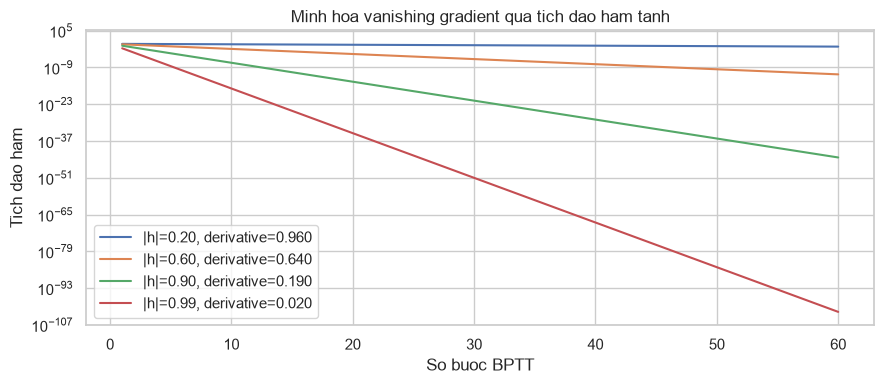
\includegraphics[width=0.88\textwidth]{rnn_vanishing_gradient.png}
    \caption{Minh họa sự suy giảm của tích đạo hàm tanh theo số bước BPTT}
    \label{fig:rnn_vanishing}
\end{figure}

Notebook giảm rủi ro bằng chuẩn hóa input, cửa sổ hữu hạn và gradient clipping với chuẩn tối đa 1.0
trong PyTorch. Dropout 0.2 regularize hidden representation; early stopping chọn weights tốt nhất.

\section{LSTM và GRU}
LSTM bổ sung cell state cùng các cổng input, forget và output để kiểm soát thông tin dài hạn.
GRU gọn hơn với update gate và reset gate. Hai biến thể thường giữ phụ thuộc xa tốt hơn vanilla RNN,
nhưng Assignment 06 dùng vanilla RNN để biểu diễn trực tiếp phương trình hồi quy cơ bản và giữ hai
framework tương đương.

% =========================================================================
% CHUONG 2
% =========================================================================
\chapter{Thiết Kế Thực Nghiệm}

\section{Dataset và nhiệm vụ}
\begin{table}[H]
\centering
\caption{Tổng quan hai dataset của Assignment 06}
\label{tab:dataset_overview}
\resizebox{\textwidth}{!}{%
\begin{tabular}{llllll}
\toprule
\textbf{Dataset} & \textbf{Số dòng} & \textbf{Khoảng thời gian} & \textbf{Target} & \textbf{Lookback} & \textbf{Tần suất} \\
\midrule
Amazon Stock Price & 6,684 & 15/05/1997--05/12/2023 & Close & 60 & Phiên giao dịch \\
Avocado Price & 18,249 & 04/01/2015--25/03/2018 & AveragePrice & 12 & Tuần \\
\bottomrule
\end{tabular}%
}
\end{table}

Amazon là một chuỗi duy nhất. Avocado là panel data gồm 54 region, hai type và 108 chuỗi độc lập.
Mục tiêu của cả hai là dự báo một bước: phiên giao dịch kế tiếp hoặc tuần kế tiếp.

\section{Split theo thời gian và chống data leakage}
Toàn bộ mẫu được sắp theo thời điểm của target rồi chia liên tiếp theo tỷ lệ xấp xỉ 80\%--10\%--10\%.
Do không trộn ngẫu nhiên, tập validation và test luôn nằm sau tập train, đúng với tình huống dự báo dữ
liệu chưa xuất hiện trong thực tế.

\begin{table}[H]
\centering
\caption{Số mẫu train, validation và test}
\label{tab:split}
\begin{tabular}{lrrr}
\toprule
\textbf{Dataset} & \textbf{Train} & \textbf{Validation} & \textbf{Test} \\
\midrule
Amazon & 5,299 & 662 & 663 \\
Avocado & 13,498 & 1,727 & 1,728 \\
\bottomrule
\end{tabular}
\end{table}

\codeinline{StandardScaler} chỉ học tham số trên phần train. Amazon cần một scaler cho chuỗi duy nhất;
Avocado dùng scaler riêng cho từng cặp region--type vì mặt bằng giá giữa các thị trường khác nhau. Khi
xử lý validation và test, notebook tái sử dụng mean và standard deviation của train thay vì fit lại.

\section{Kiến trúc và cấu hình huấn luyện}
Cả PyTorch và Keras dùng cùng pipeline:
\begin{equation}
    \text{Sequence}(L,1)
    \rightarrow \text{RNN}(64,\tanh)
    \rightarrow \text{Dropout}(0.2)
    \rightarrow \text{Linear}(1).
\end{equation}

\begin{table}[H]
\centering
\caption{Cấu hình huấn luyện chung}
\label{tab:training_config}
\begin{tabular}{ll}
\toprule
\textbf{Thành phần} & \textbf{Giá trị} \\
\midrule
Optimizer / loss & Adam $10^{-3}$ / MSE \\
Epoch & Tối đa 250, tối thiểu 30 \\
Batch size & 64 \\
Early stopping & Patience 25 theo validation loss \\
Scheduler & Factor 0.5, patience 5 \\
Regularization & Dropout 0.2, gradient clipping 1.0 \\
Random seed & 42 \\
PyTorch device & MPS nếu khả dụng, nếu không dùng CPU \\
\bottomrule
\end{tabular}
\end{table}

\section{Metric đánh giá}
Các metric được tính sau khi inverse-transform về đơn vị giá gốc:
\begin{align}
    \operatorname{MAE}&=\frac{1}{N}\sum_i|y_i-\hat y_i|,\\
    \operatorname{RMSE}&=\sqrt{\frac{1}{N}\sum_i(y_i-\hat y_i)^2},\\
    \operatorname{MAPE}&=\frac{100}{N}\sum_i\left|\frac{y_i-\hat y_i}{y_i}\right|,\\
    R^2&=1-\frac{\sum_i(y_i-\hat y_i)^2}{\sum_i(y_i-\bar y)^2}.
\end{align}
Persistence baseline dùng giá cuối cửa sổ làm giá dự báo và là đối chứng quan trọng cho time series.

% =========================================================================
% CHUONG 3
% =========================================================================
\chapter{Thực Nghiệm Trên Amazon Stock Price}

\section{Khảo sát và chất lượng dữ liệu}
Tệp Amazon gồm Date, Open, High, Low, Close, Adj Close và Volume; bước kiểm tra không phát hiện giá trị
khuyết hay bản ghi trùng. Close tăng theo xu hướng dài hạn, còn mức thay đổi theo ngày tập trung quanh 0
và có một số biến động lớn. Dù ngày lịch không cách đều vì cuối tuần và ngày nghỉ, thứ tự dòng vẫn biểu
diễn đúng các phiên giao dịch liên tiếp.

\begin{figure}[H]
    \centering
    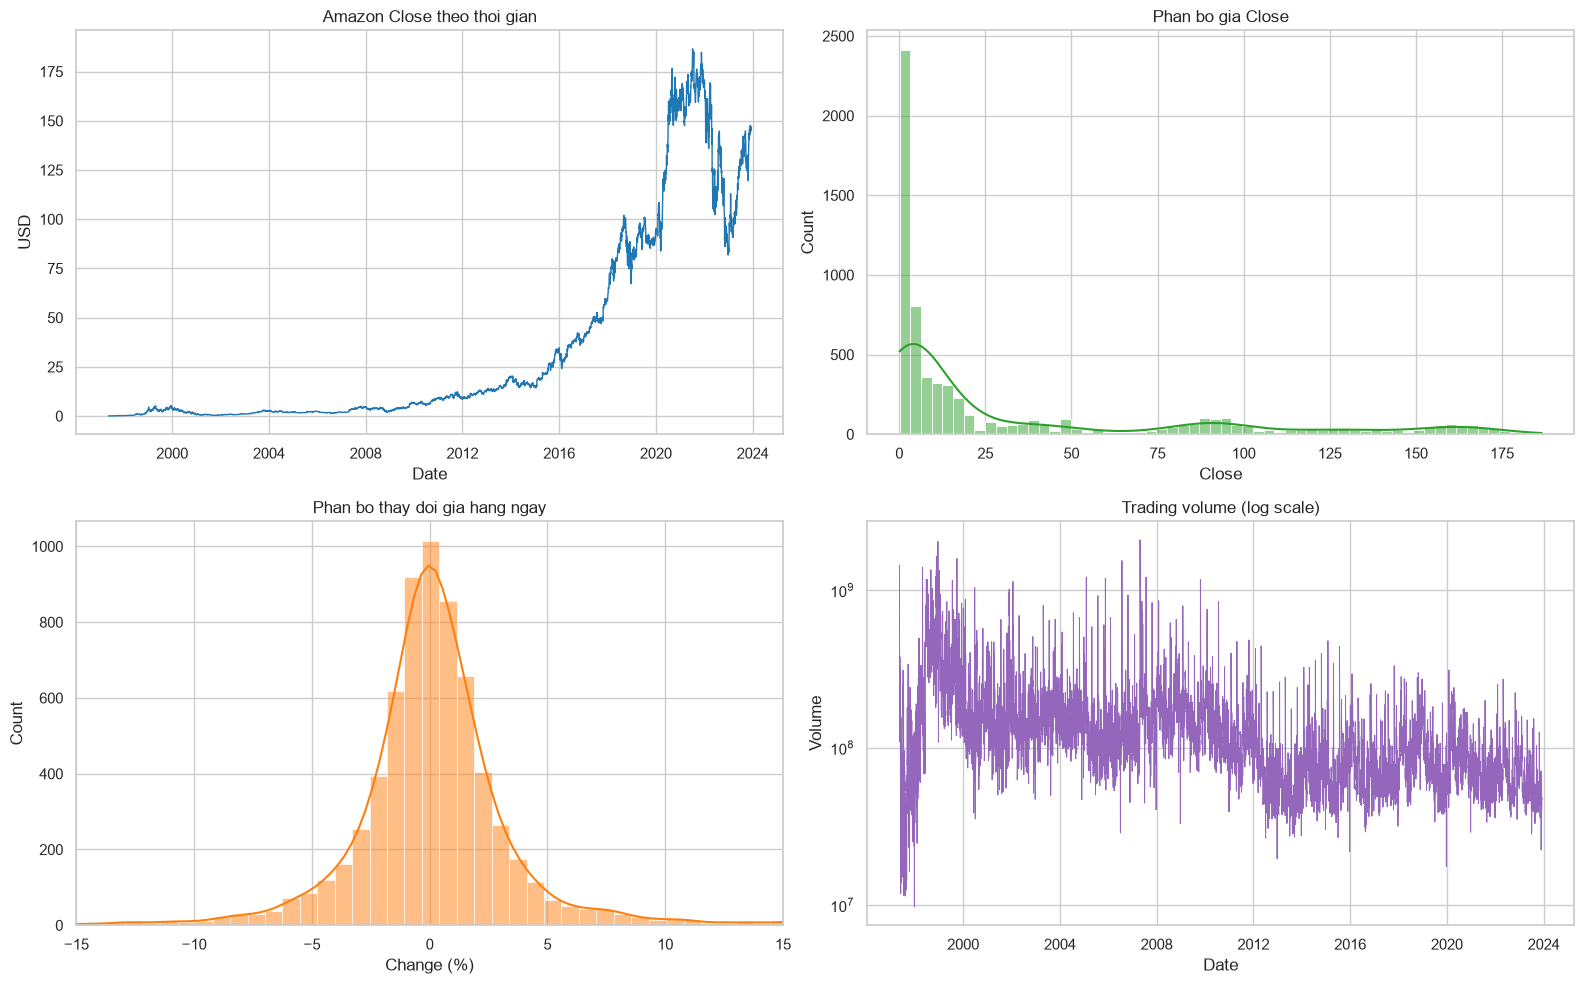
\includegraphics[width=\textwidth]{amazon_eda_overview.png}
    \caption{EDA tổng quan lịch sử giá, phân phối Close, biến động ngày và volume Amazon}
    \label{fig:amazon_eda_overview}
\end{figure}

\begin{figure}[H]
    \centering
    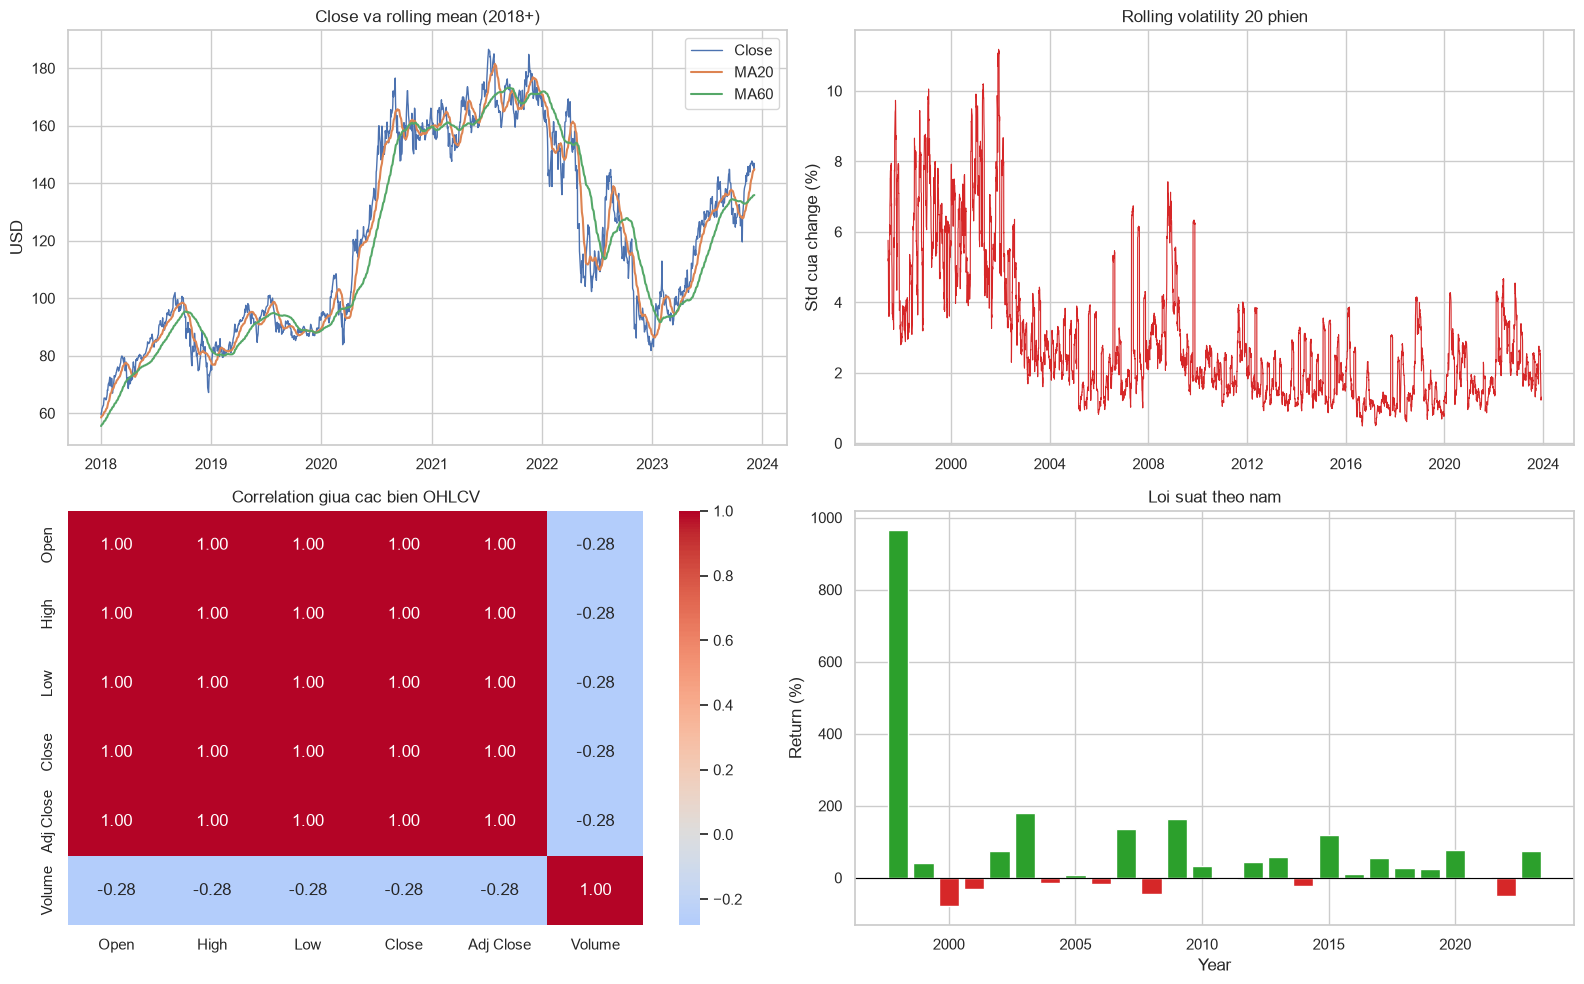
\includegraphics[width=\textwidth]{amazon_eda_diagnostics.png}
    \caption{Rolling statistics, correlation OHLCV và lợi suất năm của Amazon}
    \label{fig:amazon_eda_diagnostics}
\end{figure}

Các biến OHLC tương quan cao vì cùng phản ánh diễn biến trong một phiên. Close cũng có tự tương quan lớn,
song kết quả này chịu ảnh hưởng đáng kể của xu hướng và không đủ để kết luận chuỗi dừng. Đồ thị rolling
volatility cho thấy mức rủi ro thay đổi theo từng giai đoạn thị trường.

\section{Tạo sequence và huấn luyện}
Sau lookback 60, dataset tạo 6,624 samples. Scaler train-only có mean 11.5805 và scale 17.4447.
PyTorch chạy 107 epoch, mất 101.50 giây và lưu best validation loss 0.309872.
Keras chạy 75 epoch, mất 18.88 giây. Cả hai best weights được nạp lại độc lập trước khi test.

\section{Kết quả benchmark}
\begin{table}[H]
\centering
\caption{Kết quả test trên Amazon Stock Price}
\label{tab:amazon_results}
\resizebox{\textwidth}{!}{%
\begin{tabular}{lrrrrr}
\toprule
\textbf{Mô hình} & \textbf{MAE} & \textbf{RMSE} & \textbf{MAPE (\%)} & \textbf{$R^2$} & \textbf{Train (s)} \\
\midrule
Persistence baseline & \best{2.2720} & \best{3.1507} & \best{1.7519} & \best{0.9874} & 0.00 \\
PyTorch RNN & 10.4466 & 13.6738 & 6.7825 & 0.7633 & 101.50 \\
Keras RNN & 10.5704 & 14.1749 & 6.8377 & 0.7456 & 18.88 \\
\bottomrule
\end{tabular}%
}
\end{table}

\begin{figure}[H]
    \centering
    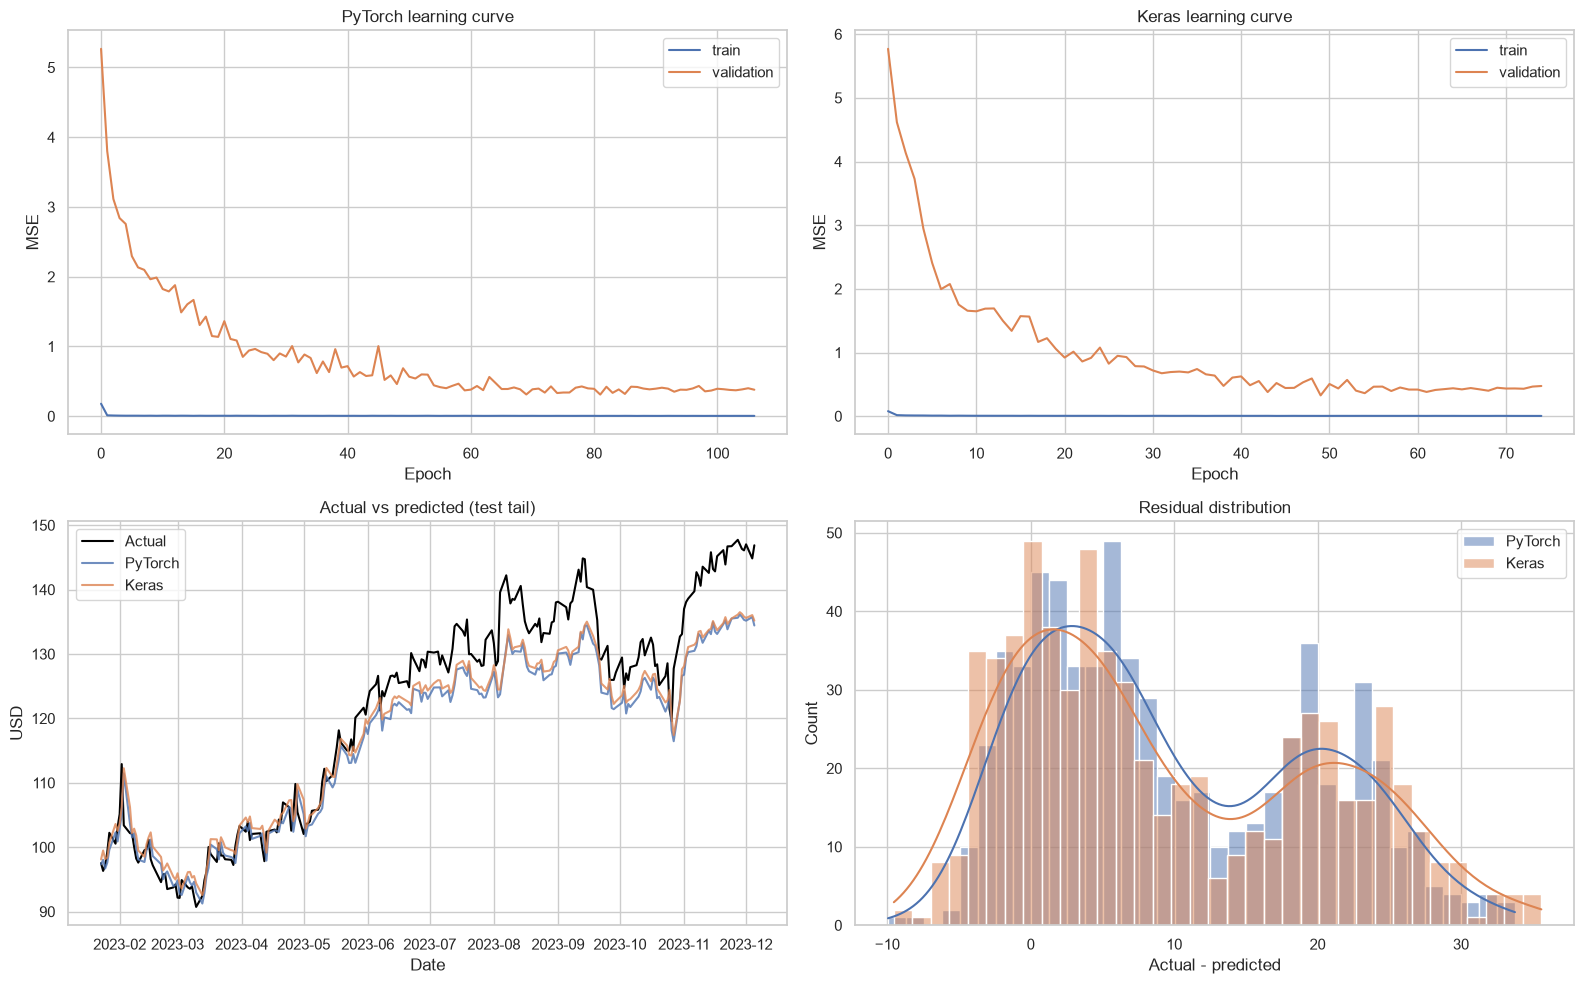
\includegraphics[width=\textwidth]{amazon_model_evaluation.png}
    \caption{Learning curves, actual--predicted và residual trên test Amazon}
    \label{fig:amazon_evaluation}
\end{figure}

Trên Amazon, quy tắc persistence đạt sai số thấp hơn cả hai RNN. Nguyên nhân hợp lý là mô hình đang học
trực tiếp mức giá có xu hướng mạnh, trong khi phần test nằm ở vùng giá cao hơn phần lớn dữ liệu train.
RNN dùng tanh vì vậy dễ kéo dự báo về miền đã quan sát; baseline lại khai thác trực tiếp tính liên tục giữa
hai phiên liền nhau. Có thể cải thiện thí nghiệm bằng return/difference, rolling normalization hoặc cơ chế
walk-forward retraining.

% =========================================================================
% CHUONG 4
% =========================================================================
\chapter{Thực Nghiệm Trên Avocado Price}

\section{Đặc điểm panel data}
Bộ dữ liệu Avocado có 18,249 dòng, trải trên 169 mốc tuần, 54 region và hai loại conventional/organic.
Tổ hợp (Date, region, type) không trùng lặp; 107 chuỗi đủ 169 quan sát, chuỗi còn lại có 166. Nhóm organic
thường có AveragePrice cao hơn conventional, còn volume phân bố lệch phải và chênh lệch đáng kể giữa vùng.

\begin{figure}[H]
    \centering
    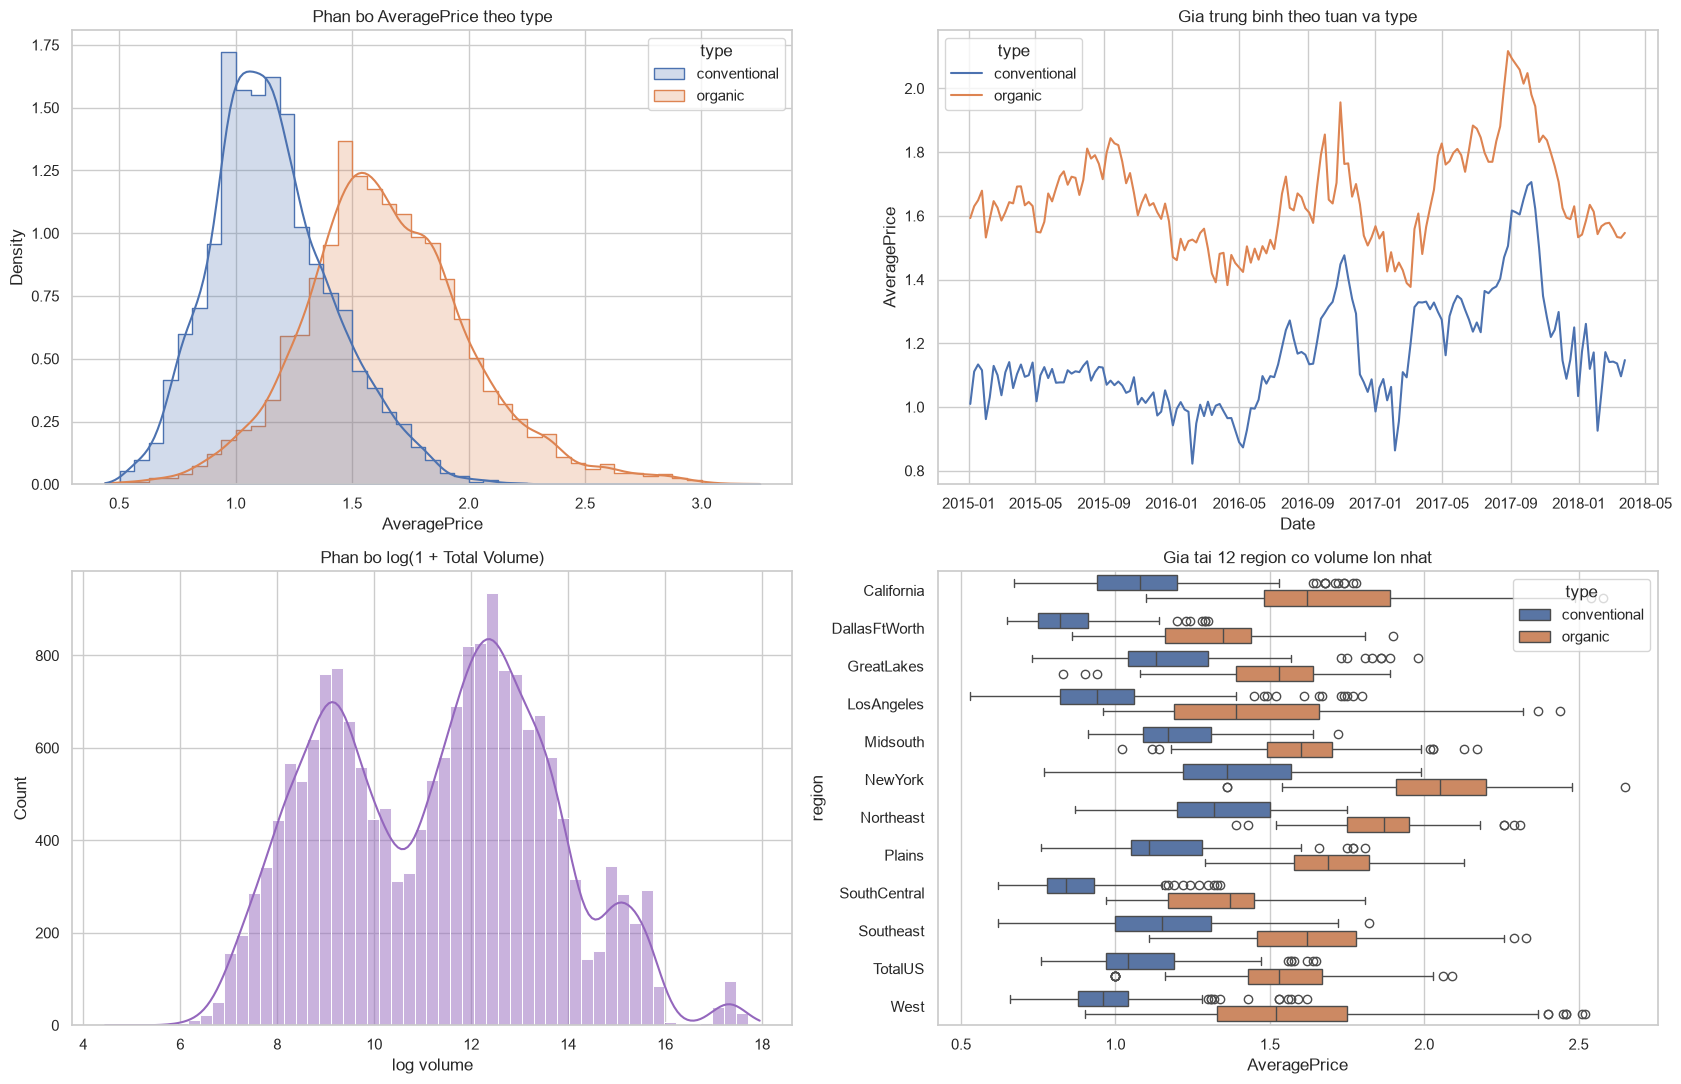
\includegraphics[width=\textwidth]{avocado_eda_overview.png}
    \caption{Phân phối giá, xu hướng tuần, volume và so sánh region của Avocado}
    \label{fig:avocado_eda_overview}
\end{figure}

\begin{figure}[H]
    \centering
    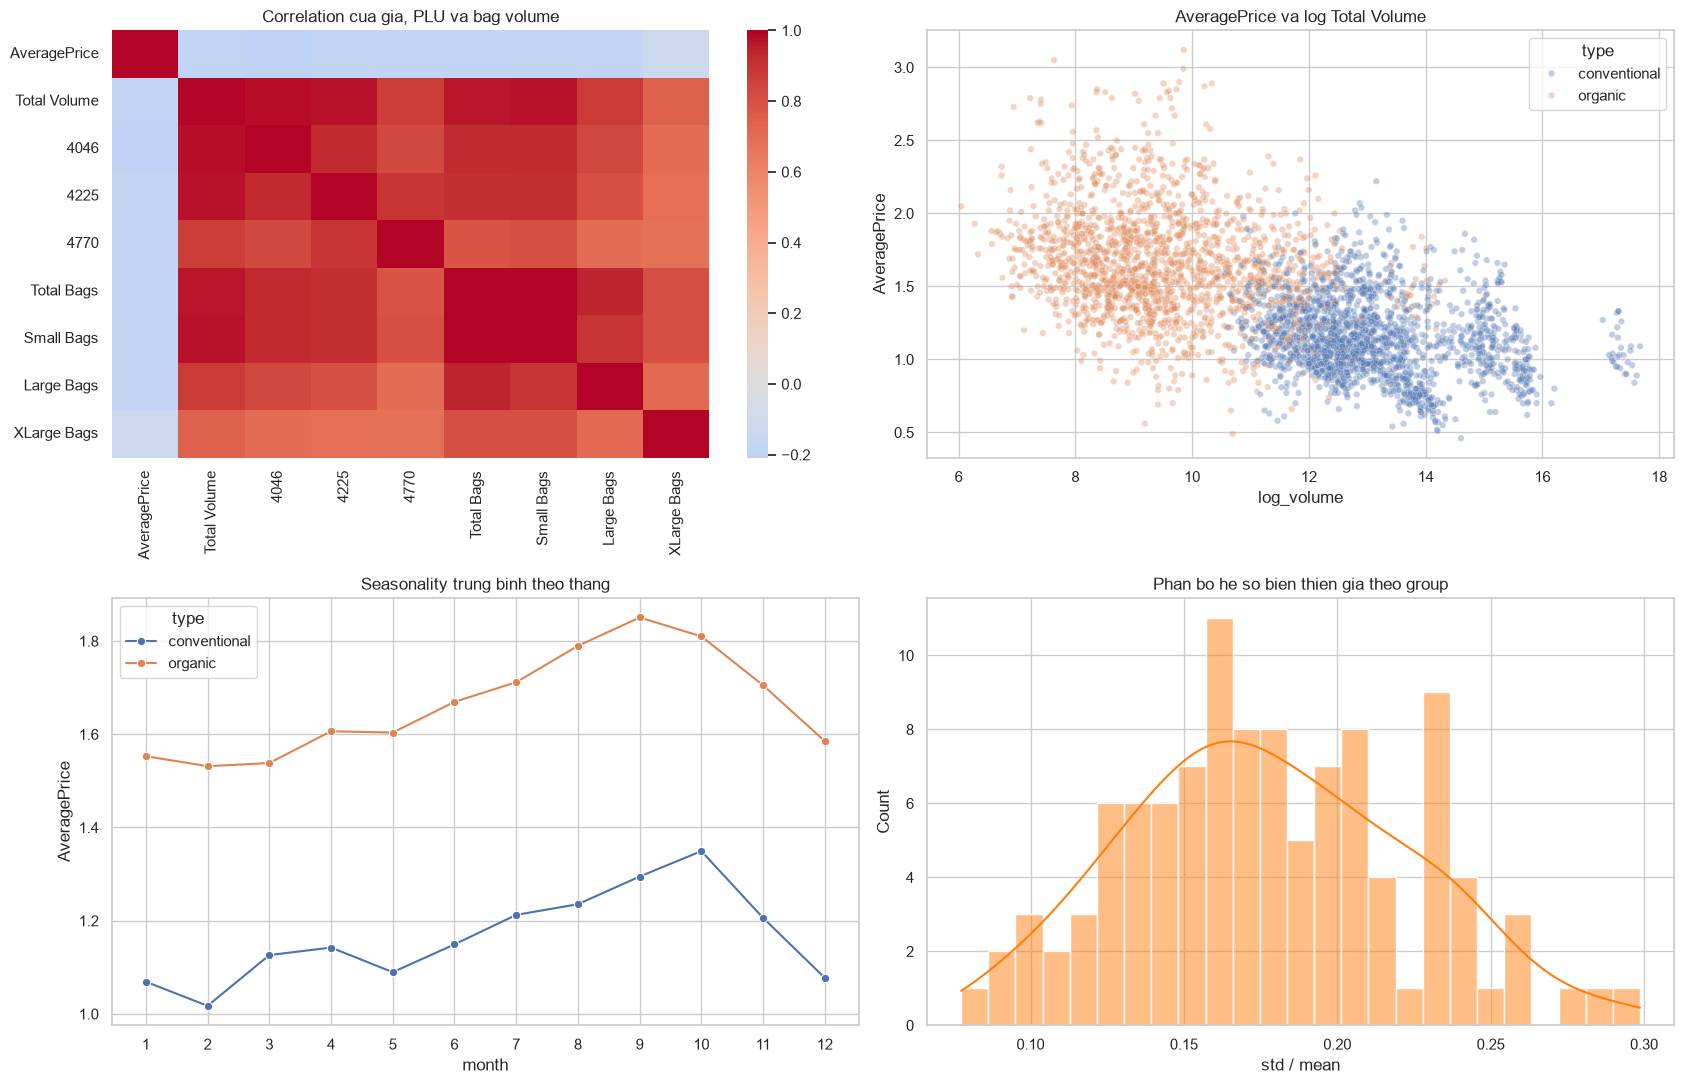
\includegraphics[width=\textwidth]{avocado_eda_diagnostics.png}
    \caption{Correlation, quan hệ giá--volume, seasonality và biến thiên theo nhóm}
    \label{fig:avocado_eda_diagnostics}
\end{figure}

Seasonality cho thấy mức giá thay đổi theo tháng và type. Correlation giữa các cột volume/PLU/bag
phản ánh cấu trúc tổng hợp của dataset; scatter giá--log volume chỉ mang ý nghĩa mô tả, không chứng minh
quan hệ nhân quả.

\section{Tạo sequence theo nhóm và huấn luyện}
Notebook tạo cửa sổ bên trong từng chuỗi region--type trước khi gộp mẫu, nhờ đó không có input nào nối
giá của hai thị trường khác nhau. Một RNN chung được huấn luyện trên dữ liệu của cả 108 nhóm. Bản PyTorch
dừng sau 32 epoch, mất 22.72 giây với validation loss tốt nhất 0.773740; bản Keras mất 10.88 giây và đạt
validation loss tốt nhất 0.877579.

\section{Kết quả benchmark}
\begin{table}[H]
\centering
\caption{Kết quả test tổng hợp trên 108 chuỗi Avocado}
\label{tab:avocado_results}
\resizebox{\textwidth}{!}{%
\begin{tabular}{lrrrrr}
\toprule
\textbf{Mô hình} & \textbf{MAE} & \textbf{RMSE} & \textbf{MAPE (\%)} & \textbf{$R^2$} & \textbf{Train (s)} \\
\midrule
Keras RNN & \best{0.1099} & \best{0.1534} & \best{8.7926} & \best{0.7490} & 10.88 \\
PyTorch RNN & 0.1122 & 0.1562 & 9.0260 & 0.7398 & 22.72 \\
Persistence baseline & 0.1199 & 0.1742 & 9.5478 & 0.6762 & 0.00 \\
\bottomrule
\end{tabular}%
}
\end{table}

\begin{figure}[H]
    \centering
    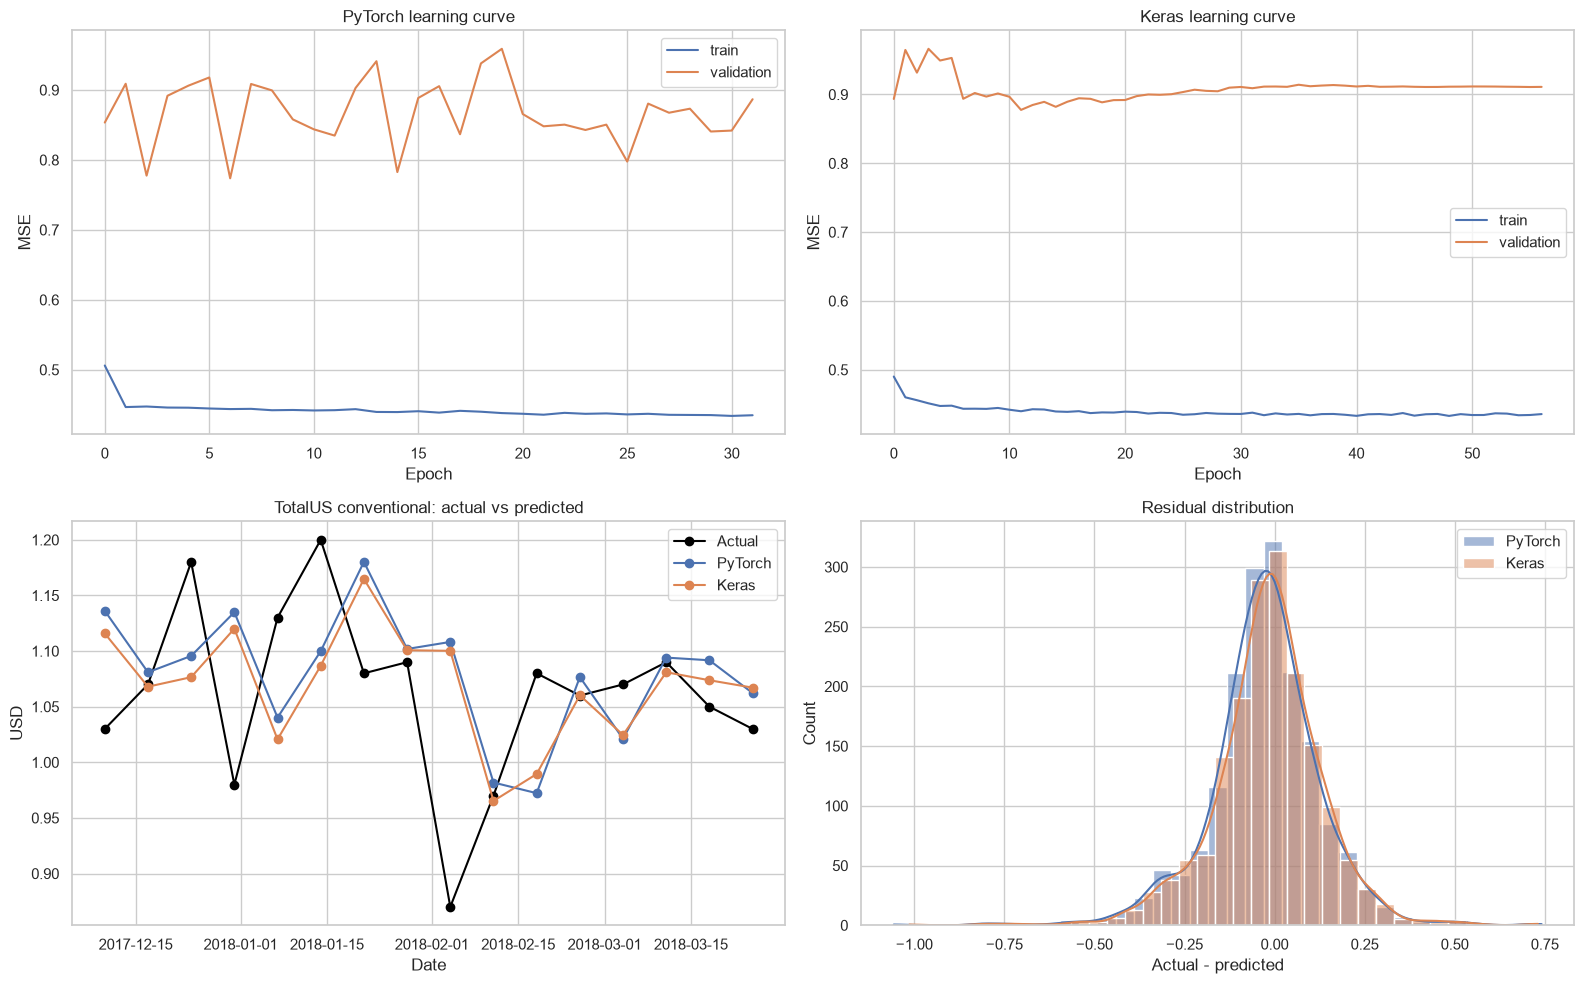
\includegraphics[width=\textwidth]{avocado_model_evaluation.png}
    \caption{Learning curves, dự báo TotalUS--conventional và residual Avocado}
    \label{fig:avocado_evaluation}
\end{figure}

Ở Avocado, cả hai RNN đều cải thiện bốn metric so với persistence. Keras dẫn đầu với RMSE 0.1534 và
$R^2=0.7490$, nhưng khoảng cách với PyTorch không lớn. Sai khác còn lại có thể xuất phát từ phép khởi tạo,
cách xử lý recurrent bias và quỹ đạo tối ưu riêng của từng framework dù cấu hình tổng thể tương đương.

% =========================================================================
% CHUONG 5
% =========================================================================
\chapter{Triển Khai Mô Hình Trên Localhost}

\section{Kiến trúc deploy}
Mỗi bài toán có một \codeinline{deploy.py} độc lập, bao gồm Flask app, giao diện HTML/CSS/JavaScript,
định nghĩa lại kiến trúc RNN và phần nạp trọng số. Một request dự báo đi qua chuỗi xử lý:
\begin{equation}
    \text{Web input}
    \rightarrow \text{Validate}
    \rightarrow \text{Scale}
    \rightarrow \text{RNN inference}
    \rightarrow \text{Inverse scale}
    \rightarrow \text{JSON/UI result}.
\end{equation}
Mô hình được cache sau lần nạp đầu tiên để các request tiếp theo không phải đọc lại weights. PyTorch chọn
MPS khi thiết bị hỗ trợ và chuyển về CPU trong trường hợp còn lại; Keras dùng thiết bị do TensorFlow phát
hiện. Cả hai server mặc định chỉ bind \codeinline{127.0.0.1} nên chỉ phục vụ trên máy đang chạy.

\section{Đầu vào và API}
\begin{table}[H]
\centering
\caption{Đầu vào của hai ứng dụng deploy}
\label{tab:deploy_inputs}
\resizebox{\textwidth}{!}{%
\begin{tabular}{lllll}
\toprule
\textbf{Ứng dụng} & \textbf{Framework} & \textbf{Chuỗi giá} & \textbf{Thông tin thêm} & \textbf{Đầu ra} \\
\midrule
Amazon & pytorch / keras & 60 giá Close, cũ $\to$ mới & Không & Close phiên kế tiếp \\
Avocado & pytorch / keras & 12 AveragePrice, cũ $\to$ mới & region, type & AveragePrice tuần kế tiếp \\
\bottomrule
\end{tabular}%
}
\end{table}

Amazon cung cấp \codeinline{POST /api/predict}. Avocado có thêm
\codeinline{GET /api/latest} để đọc 12 tuần mới nhất của nhóm được chọn.
Backend từ chối sai lookback, giá âm, số không hữu hạn, framework hoặc region--type không hợp lệ.

\clearpage
\thispagestyle{fancy}
\section{Giao diện Amazon}
\begin{figure}[H]
    \centering
    \safeimage{amazon_deploy_result.png}{Ảnh giao diện Amazon deploy sau khi dự báo}
    \caption{Giao diện localhost Amazon sau khi dự báo bằng PyTorch}
    \label{fig:amazon_deploy}
\end{figure}

Giao diện tự nạp 60 giá Close cuối từ \codeinline{AMZN.csv}, cho phép đổi framework và hiển thị giá dự
báo cùng device inference. Cổng mặc định là 8001.

\clearpage
\thispagestyle{fancy}
\vspace*{0.5cm}
\section{Giao diện Avocado}
\begin{figure}[H]
    \centering
    \safeimage[0.85\textwidth]{avocado_deploy_result.png}{Ảnh giao diện Avocado deploy sau khi dự báo}
    \caption{Giao diện localhost Avocado cho TotalUS--conventional sau khi dự báo bằng PyTorch}
    \label{fig:avocado_deploy}
\end{figure}

Giao diện cho phép chọn 54 region, hai type và framework. Khi region/type thay đổi, 12 tuần gần nhất
được nạp lại theo nhóm. Cổng mặc định là 8002.

\section{Cách chạy}
Từ thư mục gốc project, kích hoạt môi trường và chạy hai terminal:
\begin{lstlisting}[language=bash,caption={Khởi động hai web deploy trên localhost}]
conda activate ISD
    python "Assignment6/Amazon Stock Price/deploy.py" --web
    python "Assignment6/Avocado Price/deploy.py" --web
\end{lstlisting}
Sau đó mở một trong hai địa chỉ sau:
\begin{itemize}
    \item Amazon: \url{http://127.0.0.1:8001};
    \item Avocado: \url{http://127.0.0.1:8002}.
\end{itemize}
Dừng server bằng \codeinline{Ctrl+C}. CLI vẫn được giữ để tích hợp tự động hoặc kiểm thử không giao diện.

% =========================================================================
% CHUONG 6
% =========================================================================
\chapter{Tổng Hợp Và Kết Luận}

\section{Tổng hợp kết quả}
\begin{table}[H]
\centering
\caption{Mô hình có RMSE thấp nhất trong từng dataset}
\label{tab:master_summary}
\begin{tabular}{llrrrr}
\toprule
\textbf{Dataset} & \textbf{Mô hình} & \textbf{MAE} & \textbf{RMSE} & \textbf{MAPE (\%)} & \textbf{$R^2$} \\
\midrule
Amazon & Persistence baseline & 2.2720 & 3.1507 & 1.7519 & 0.9874 \\
Avocado & Keras RNN & 0.1099 & 0.1534 & 8.7926 & 0.7490 \\
\bottomrule
\end{tabular}
\end{table}

Hai dataset cho hai kết luận khác nhau. Với Amazon, persistence là đối chứng bắt buộc vì một mô hình phức
tạp chưa chắc vượt quy tắc giữ nguyên giá gần nhất. Với Avocado, RNN huấn luyện chung sau khi chuẩn hóa
riêng từng nhóm đã học được biến động theo tuần và tạo ra cải thiện thực sự so với baseline.

\section{Kiểm toán khả năng tái lập}
\begin{table}[H]
\centering
\caption{Checklist tái lập Assignment 06}
\label{tab:reproducibility}
\resizebox{\textwidth}{!}{%
\begin{tabular}{lll}
\toprule
\textbf{Hạng mục} & \textbf{Cách thực hiện} & \textbf{Ý nghĩa} \\
\midrule
Random seed & Seed 42 cho NumPy, Python, PyTorch, Keras & Giảm dao động khởi tạo \\
Split & Theo target time 80/10/10, không shuffle giữa tập & Không nhìn tương lai \\
Scaling & Fit chỉ trên train; Avocado theo nhóm & Chống data leakage \\
Thiết bị & MPS ưu tiên, CPU fallback & Tận dụng Apple Silicon \\
Checkpoint & Lưu best validation loss & Deploy weights tốt nhất \\
Reload test & Dự đoán sau reload khớp notebook & Xác nhận artifact dùng được \\
Baseline & Persistence trên cùng test set & Đối chứng thực tế \\
Deploy test & Flask page/API và lỗi input & Kiểm chứng inference end-to-end \\
\bottomrule
\end{tabular}%
}
\end{table}

\section{Giới hạn và hướng mở rộng}
\begin{itemize}
    \item Amazon dùng mức giá chưa dừng và scaler cố định từ train; nên thử return, difference,
          walk-forward validation và rolling normalization.
    \item Vanilla RNN có hạn chế về phụ thuộc dài; có thể benchmark thêm LSTM, GRU và attention.
    \item Hai mô hình chỉ dùng lịch sử giá; có thể bổ sung volume, OHLCV, calendar features và biến ngoại sinh.
    \item Cần chạy nhiều seed và báo cáo mean $\pm$ standard deviation để đánh giá độ ổn định.
    \item Flask development server phù hợp localhost; triển khai nhiều người dùng cần WSGI server,
          authentication, logging và giới hạn request.
\end{itemize}

\section{Kết luận}
Assignment 06 đã hoàn thiện quy trình dự báo một bước bằng vanilla RNN cho một chuỗi đơn và dữ liệu panel.
Hai phiên bản PyTorch/Keras được đánh giá bằng split thời gian, lưu checkpoint tốt nhất và tái sử dụng trong
ứng dụng web localhost. Kết quả Avocado cho thấy RNN có thể vượt persistence khi dữ liệu được tách và scale
đúng theo nhóm; trường hợp Amazon lại chỉ ra rằng cách biểu diễn chuỗi và baseline có ảnh hưởng lớn hơn độ
phức tạp của mô hình. Notebook, weights, metadata, chế độ CLI và Flask app hiện liên kết thành một quy trình
nhất quán từ phân tích dữ liệu đến suy luận.

\end{document}
